%==============================================================================
% Concrete Example: Python Code → Transition System → Polynomial Certificate
% via Barrier-Theoretic Verification
%==============================================================================

\documentclass[11pt,a4paper]{article}

\usepackage[utf8]{inputenc}
\usepackage[T1]{fontenc}
\usepackage{amsmath,amssymb,amsthm}
\usepackage{stmaryrd}
\usepackage{mathtools}
\usepackage{tikz}
\usetikzlibrary{positioning,arrows.meta,shapes.geometric,calc,
  decorations.pathmorphing,backgrounds,fit,patterns}
\usepackage{hyperref}
\usepackage{cleveref}
\usepackage{booktabs}
\usepackage{enumitem}
\usepackage{geometry}
\usepackage{listings}
\usepackage{xcolor}
\usepackage{pifont}
\usepackage{pgfplots}
\pgfplotsset{compat=1.18}
\usepackage{mdframed}

\geometry{margin=1in}

% Theorem environments
\theoremstyle{plain}
\newtheorem{theorem}{Theorem}[section]
\newtheorem{lemma}[theorem]{Lemma}
\newtheorem{proposition}[theorem]{Proposition}
\newtheorem{corollary}[theorem]{Corollary}

\theoremstyle{definition}
\newtheorem{definition}[theorem]{Definition}
\newtheorem{example}[theorem]{Example}
\newtheorem{construction}[theorem]{Construction}

\theoremstyle{remark}
\newtheorem{remark}[theorem]{Remark}

% Notation
\newcommand{\R}{\mathbb{R}}
\newcommand{\Z}{\mathbb{Z}}
\newcommand{\N}{\mathbb{N}}
\newcommand{\StateSpace}{\mathcal{S}}
\newcommand{\Reach}{\operatorname{Reach}}
\newcommand{\Init}{\operatorname{Init}}
\newcommand{\Trans}{\operatorname{Trans}}
\newcommand{\Unsafe}{\operatorname{Unsafe}}
\newcommand{\sem}[1]{\llbracket #1 \rrbracket}

% Python listings
\lstdefinestyle{python}{
  language=Python,
  basicstyle=\ttfamily\small,
  keywordstyle=\color{blue!70!black}\bfseries,
  commentstyle=\color{green!50!black}\itshape,
  stringstyle=\color{red!60!black},
  showstringspaces=false,
  breaklines=true,
  frame=single,
  framerule=0.5pt,
  rulecolor=\color{gray!40},
  backgroundcolor=\color{gray!5},
  numbers=left,
  numberstyle=\tiny\color{gray},
  numbersep=6pt,
  xleftmargin=2em,
  framexleftmargin=1.5em,
  tabsize=4,
  morekeywords={cursor,execute,escape_string,request}
}

% Bytecode listings
\lstdefinestyle{bytecode}{
  basicstyle=\ttfamily\scriptsize,
  frame=single,
  framerule=0.5pt,
  rulecolor=\color{gray!40},
  backgroundcolor=\color{blue!3},
  numbers=left,
  numberstyle=\tiny\color{gray},
  numbersep=6pt,
  xleftmargin=2em,
  framexleftmargin=1.5em,
}

% Colored boxes
\newmdenv[
  linecolor=blue!60!black,
  backgroundcolor=blue!5!white,
  linewidth=1pt,
  roundcorner=3pt,
  innertopmargin=10pt,
  innerbottommargin=10pt,
  frametitle={\textbf{Key Insight}},
  frametitlebackgroundcolor=blue!15
]{keyinsight}

\newmdenv[
  linecolor=red!60!black,
  backgroundcolor=red!5!white,
  linewidth=1pt,
  roundcorner=3pt,
  innertopmargin=10pt,
  innerbottommargin=10pt,
  frametitle={\textbf{Why Non-Barrier Approaches Fail}},
  frametitlebackgroundcolor=red!15
]{whybarrier}

\newmdenv[
  linecolor=green!50!black,
  backgroundcolor=green!5!white,
  linewidth=1pt,
  roundcorner=3pt,
  innertopmargin=10pt,
  innerbottommargin=10pt,
  frametitle={\textbf{Barrier Certificate Proof}},
  frametitlebackgroundcolor=green!15
]{barrierproof}

\newmdenv[
  linecolor=blue!70!black,
  backgroundcolor=blue!5!white,
  linewidth=1.5pt,
  roundcorner=3pt,
  innertopmargin=10pt,
  innerbottommargin=10pt,
  frametitle={\textbf{Complete Pipeline: Python $\to$ Transition System $\to$ Polynomial Certificate}},
  frametitlebackgroundcolor=blue!15
]{pipelinebox}
\title{%
  \textbf{From Python to Polynomial Certificates} \\[0.4em]
  \Large A Concrete Barrier-Theoretic Verification \\
  of Interprocedural Taint Safety \\[0.5em]
  \large SQL Injection $\cdot$ Taint Lattices $\cdot$ Compositional Barriers
}

\author{A3 Python Verification Framework}
\date{March 2026}

\begin{document}
\maketitle

\begin{abstract}
We present a complete, concrete example of mapping Python source code
through bytecode to a polynomial transition system, and synthesizing a
barrier certificate that proves freedom from SQL injection.  This is a
property where barrier certificates are \emph{strictly more powerful}
than type checking, standard abstract interpretation, or bounded model
checking: the barrier provides a compositional, interprocedural
separation proof that no finite unrolling or conservative
type-based analysis can replicate.  We give every equation, every
state variable, and every diagram, from the Python source to the final
SOS certificate.
\end{abstract}

\tableofcontents
\newpage

%==============================================================================
\section{The Running Example: SQL Injection with Sanitization}
\label{sec:example}
%==============================================================================

\subsection{Python Source Code}

Consider the following web-application function that queries a database
using user-supplied input:

\begin{lstlisting}[style=python, caption={Target Python function}, label=lst:target]
def search_users(request, cursor):
    """Search users by name from HTTP request."""
    raw_name = request.args.get("name")      # TAINT SOURCE
    if raw_name is None:
        return []

    clean_name = escape_string(raw_name)      # SANITIZER

    query = "SELECT * FROM users WHERE name = '%s'" % clean_name
    cursor.execute(query)                     # SINK
    return cursor.fetchall()
\end{lstlisting}

\noindent
The question: \emph{Is this function safe from SQL injection (CWE-089)?}

\medskip
There is also an unsafe variant:
\begin{lstlisting}[style=python, caption={Unsafe variant (no sanitizer)}, label=lst:unsafe]
def search_users_unsafe(request, cursor):
    raw_name = request.args.get("name")       # TAINT SOURCE
    if raw_name is None:
        return []

    query = "SELECT * FROM users WHERE name = '%s'" % raw_name
    cursor.execute(query)                     # SINK: VULNERABLE!
    return cursor.fetchall()
\end{lstlisting}

\subsection{The Verification Challenge}

\begin{whybarrier}
\textbf{Type checking} cannot distinguish a tainted \texttt{str} from a
clean \texttt{str}.  Both have type \texttt{str}; the type system has no
refinement to capture ``sanitized.''

\textbf{Standard abstract interpretation} with a taint domain must
conservatively havoc at unknown function calls.  When
\texttt{escape\_string} is an opaque library function, the abstract
interpreter must assume the return value \emph{might} still be tainted
(it cannot prove the function removes taint without analyzing it).

\textbf{Bounded model checking} (BMC) can unroll a fixed number of paths, but:
\begin{enumerate}[nosep]
  \item It cannot prove safety for \emph{all} inputs (only for explored paths).
  \item Interprocedural BMC requires inlining all callees, which does not scale.
  \item It provides no reusable proof artifact.
\end{enumerate}

\textbf{Barrier certificates} provide a \emph{compositional separation
proof}: a polynomial function $B$ over the state variables that is
non-negative on all reachable states and negative on all unsafe states.
The barrier composes across function boundaries via assume-guarantee
contracts, needs no inlining, and serves as a checkable proof artifact.
\end{whybarrier}

%==============================================================================
\section{Step 1: Python $\to$ Bytecode $\to$ Control Flow Graph}
\label{sec:cfg}
%==============================================================================

\subsection{Bytecode Extraction}

The A3 framework compiles the source to CPython 3.12+ bytecode and
extracts a control flow graph.  The relevant bytecode for
Listing~\ref{lst:target} (simplified) is:

\begin{lstlisting}[style=bytecode, caption={Simplified bytecode for \texttt{search\_users}}]
  0: LOAD_FAST        request           # push request
  2: LOAD_ATTR        args              # request.args
  4: LOAD_ATTR        get               # request.args.get
  6: LOAD_CONST       "name"
  8: CALL             1                 # raw_name = request.args.get("name")
 10: STORE_FAST       raw_name
 12: LOAD_FAST        raw_name
 14: POP_JUMP_IF_NOT_NONE  20           # if raw_name is None:
 16: BUILD_LIST       0                 #   return []
 18: RETURN_VALUE
 20: LOAD_GLOBAL      escape_string     # clean_name = escape_string(raw_name)
 22: LOAD_FAST        raw_name
 24: CALL             1
 26: STORE_FAST       clean_name
 28: LOAD_CONST       "SELECT...%s"
 30: LOAD_FAST        clean_name
 32: BINARY_OP        MOD               # query = "..." % clean_name
 34: STORE_FAST       query
 36: LOAD_FAST        cursor
 38: LOAD_ATTR        execute
 40: LOAD_FAST        query
 42: CALL             1                 # cursor.execute(query)
 44: POP_TOP
 46: LOAD_FAST        cursor
 48: LOAD_ATTR        fetchall
 50: CALL             0
 52: RETURN_VALUE
\end{lstlisting}

\subsection{Control Flow Graph}

\begin{figure}[ht]
\centering
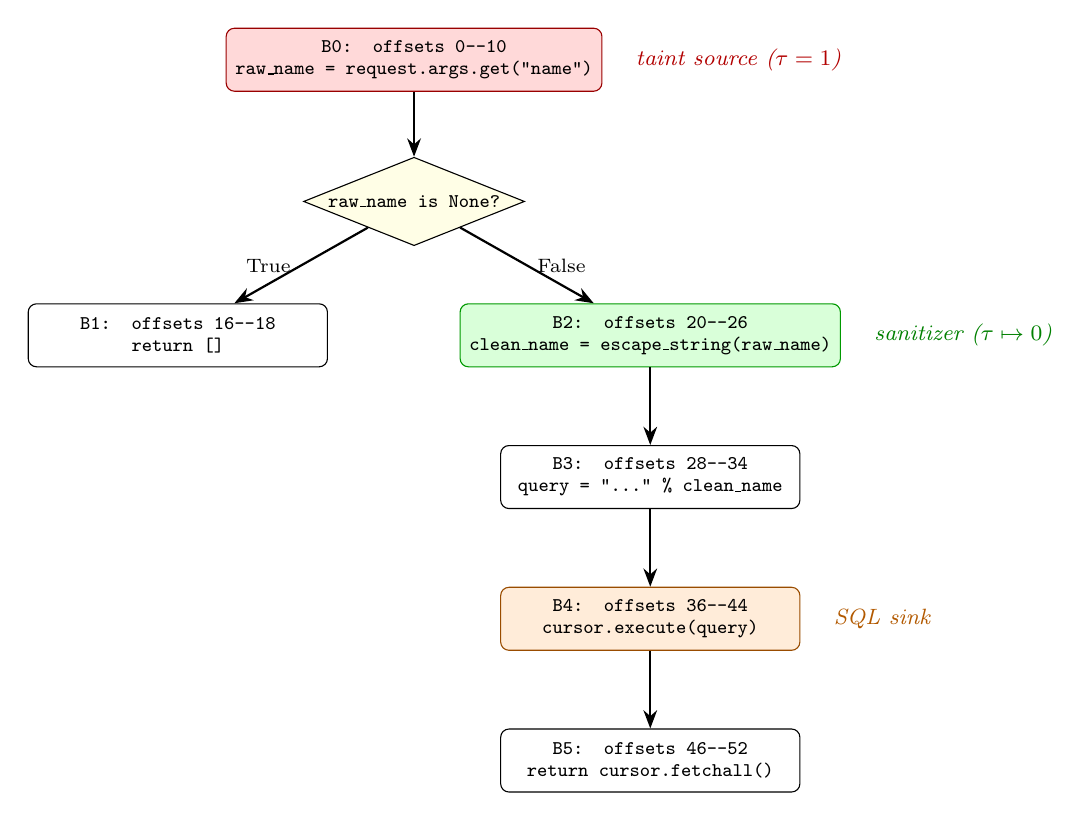
\begin{tikzpicture}[
  block/.style={
    rectangle, draw, rounded corners=3pt,
    minimum width=3.8cm, minimum height=0.8cm,
    font=\ttfamily\scriptsize, align=center,
    fill=white
  },
  source/.style={block, fill=red!15, draw=red!60!black},
  sanitizer/.style={block, fill=green!15, draw=green!60!black},
  sink/.style={block, fill=orange!15, draw=orange!60!black},
  guard/.style={diamond, draw, aspect=2.5, inner sep=1pt,
    font=\ttfamily\scriptsize, fill=yellow!10},
  arr/.style={-Stealth, thick},
  every edge quotes/.style={font=\scriptsize, auto, inner sep=2pt}
]

% Blocks
\node[source] (B0) at (0,0) {B0: offsets 0--10\\
  \texttt{raw\_name = request.args.get("name")}};

\node[guard] (G1) at (0,-1.8) {\texttt{raw\_name is None?}};

\node[block] (B1) at (-3,-3.5) {B1: offsets 16--18\\
  \texttt{return []}};

\node[sanitizer] (B2) at (3,-3.5) {B2: offsets 20--26\\
  \texttt{clean\_name = escape\_string(raw\_name)}};

\node[block] (B3) at (3,-5.3) {B3: offsets 28--34\\
  \texttt{query = "..." \% clean\_name}};

\node[sink] (B4) at (3,-7.1) {B4: offsets 36--44\\
  \texttt{cursor.execute(query)}};

\node[block] (B5) at (3,-8.9) {B5: offsets 46--52\\
  \texttt{return cursor.fetchall()}};

% Edges
\draw[arr] (B0) -- (G1);
\draw[arr] (G1) -- node[left,font=\scriptsize] {True} (B1);
\draw[arr] (G1) -- node[right,font=\scriptsize] {False} (B2);
\draw[arr] (B2) -- (B3);
\draw[arr] (B3) -- (B4);
\draw[arr] (B4) -- (B5);

% Annotations
\node[right=0.3cm of B0, red!70!black, font=\footnotesize\itshape] {taint source ($\tau=1$)};
\node[right=0.3cm of B2, green!50!black, font=\footnotesize\itshape] {sanitizer ($\tau \mapsto 0$)};
\node[right=0.3cm of B4, orange!70!black, font=\footnotesize\itshape] {SQL sink};

\end{tikzpicture}
\caption{Control flow graph for \texttt{search\_users}.  Red = taint
  source, green = sanitizer, orange = SQL execution sink.}
\label{fig:cfg}
\end{figure}

%==============================================================================
\section{Step 2: Transition System Encoding}
\label{sec:transition}
%==============================================================================

\subsection{State Space}

Following the \texttt{step\_relation.py} module of the A3 framework,
we model the machine state as:

\begin{definition}[Taint-Augmented Machine State]
A state $s \in \StateSpace \subseteq \R^5$ is a tuple:
\[
  s = (\pi,\; \tau,\; \kappa,\; \nu,\; \rho)
\]
where:
\begin{itemize}[nosep]
  \item $\pi \in \{0,1,\ldots,5\}$ is the \emph{program counter}
    (basic block index),
  \item $\tau \in [0,1]$ is the \emph{taint level} of the data
    flowing toward the SQL sink
    ($0$ = clean, $1$ = tainted by untrusted source),
  \item $\kappa \in [0,1]$ is the \emph{sanitization flag}
    ($1$ = sanitizer has been applied, $0$ = not yet),
  \item $\nu \in \{0,1\}$ is the \emph{null flag}
    ($1$ = \texttt{raw\_name is None}, $0$ = not None),
  \item $\rho \in \{0,1\}$ is the \emph{parameterization flag}
    ($1$ = query uses parameterized execution, $0$ = string formatting).
\end{itemize}
\end{definition}

\begin{remark}
The key lifting from discrete types to $\R^n$:  Python's \texttt{str}
type carries no taint information, but our \emph{semantic} state
augments each value with a real-valued taint coordinate $\tau$.  This
is the information that type systems cannot express.
\end{remark}

\subsection{Initial States}

\begin{definition}[Initial Region]
The initial states encode function entry with an untrusted HTTP
parameter:
\begin{equation}
  \Init = \bigl\{(\pi,\tau,\kappa,\nu,\rho) :
    \pi = 0,\;
    \tau = 1,\;
    \kappa = 0,\;
    \nu \in \{0,1\},\;
    \rho = 0
  \bigr\}
\end{equation}
In polynomial form:
\begin{equation}
  \Init = \bigl\{s \in \R^5 :
    \pi^2 = 0,\;
    (\tau - 1)^2 = 0,\;
    \kappa^2 = 0,\;
    \nu(1-\nu) = 0,\;
    \rho^2 = 0
  \bigr\}
\end{equation}
\end{definition}

\subsection{Transition Relation}

The transition relation encodes the effect of each CFG edge on the
state variables.  Each edge $e_i : B_j \to B_k$ defines a
semialgebraic relation $T_i \subseteq \StateSpace \times \StateSpace$.

\begin{definition}[Transition Relations]
\label{def:transitions}
\begin{align}
  T_{\text{source}} &: (\pi=0) \;\longrightarrow\;
    (\pi'=1,\; \tau'=\tau,\; \kappa'=\kappa,\; \rho'=\rho)
    \label{eq:t-source} \\[3pt]
%
  T_{\text{null-yes}} &: (\pi=1 \;\wedge\; \nu=1) \;\longrightarrow\;
    (\pi'=\text{exit},\; \tau'=0)
    \tag{early return} \\[3pt]
%
  T_{\text{null-no}} &: (\pi=1 \;\wedge\; \nu=0) \;\longrightarrow\;
    (\pi'=2,\; \tau'=\tau)
    \label{eq:t-guard} \\[3pt]
%
  T_{\text{sanitize}} &: (\pi=2) \;\longrightarrow\;
    \bigl(\pi'=3,\; \boxed{\tau'=0},\; \kappa'=1\bigr)
    \label{eq:t-sanitize} \\[3pt]
%
  T_{\text{format}} &: (\pi=3) \;\longrightarrow\;
    (\pi'=4,\; \tau'=\tau,\; \rho'=0)
    \label{eq:t-format} \\[3pt]
%
  T_{\text{execute}} &: (\pi=4) \;\longrightarrow\;
    (\pi'=5,\; \tau'=\tau,\; \rho'=\rho)
    \label{eq:t-execute}
\end{align}
The full transition relation is the disjunction:
\begin{equation}
  \Trans(s, s') = \bigvee_i T_i(s, s')
\end{equation}
\end{definition}

\begin{keyinsight}
The critical transition is \eqref{eq:t-sanitize}: the sanitizer
\texttt{escape\_string} sets $\tau' = 0$.  This models the
\texttt{SanitizerContract} from the A3 framework's
\texttt{security\_lattice.py}, which maps sanitizer functions to the
set of sink types they clear.  In the taint lattice, this corresponds
to the join operation:
\[
  \ell_{\text{ret}} = (\tau_{\text{in}},\, \kappa_{\text{in}},\,
  \sigma_{\text{in}}) \;\mapsto\;
  (0,\, \kappa_{\text{in}} \cup \{\texttt{SQL\_EXECUTE}\},\, \sigma_{\text{in}})
\]
A type system sees both values as \texttt{str}; the barrier sees $\tau$
drop from 1 to 0.
\end{keyinsight}

\subsection{Unsafe Region}

\begin{definition}[SQL Injection Unsafe Region]
A state is unsafe if we are at the SQL execution sink with tainted,
non-parameterized data:
\begin{equation}
  \Unsafe_{\text{SQLi}} = \bigl\{s :
    \pi = 4 \;\wedge\;
    \tau = 1 \;\wedge\;
    \rho = 0
  \bigr\}
\end{equation}
In polynomial form (a product of non-negativity constraints):
\begin{equation}
  \Unsafe_{\text{SQLi}} = \bigl\{s :
    (\pi - 4)^2 = 0 \;\wedge\;
    (\tau - 1)^2 = 0 \;\wedge\;
    \rho^2 = 0
  \bigr\}
\end{equation}
\end{definition}

\subsection{Transition System Diagram}

\begin{figure}[ht]
\centering
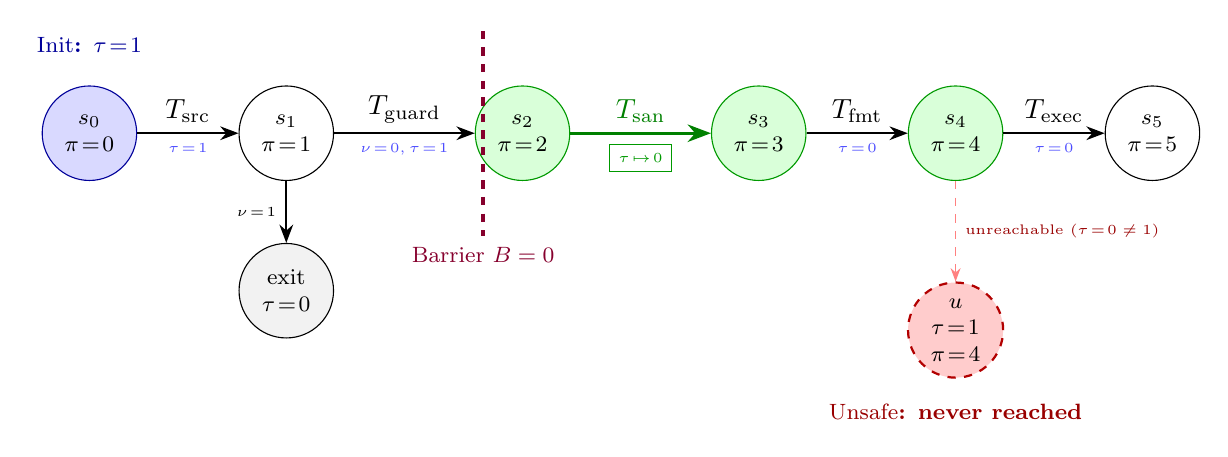
\begin{tikzpicture}[
  state/.style={
    circle, draw, minimum size=1.2cm,
    font=\footnotesize, inner sep=2pt, align=center
  },
  safe/.style={state, fill=green!15, draw=green!60!black},
  unsafe/.style={state, fill=red!20, draw=red!70!black, thick},
  init/.style={state, fill=blue!15, draw=blue!60!black},
  arr/.style={-Stealth, thick},
  every edge quotes/.style={font=\tiny, auto, inner sep=1pt}
]

% States as circles
\node[init] (s0) at (0,0) {$s_0$\\$\pi\!=\!0$};
\node[state] (s1) at (2.5,0) {$s_1$\\$\pi\!=\!1$};
\node[state, fill=gray!10] (sexit) at (2.5,-2) {exit\\$\tau\!=\!0$};
\node[safe] (s2) at (5.5,0) {$s_2$\\$\pi\!=\!2$};
\node[safe] (s3) at (8.5,0) {$s_3$\\$\pi\!=\!3$};
\node[safe] (s4) at (11,0) {$s_4$\\$\pi\!=\!4$};
\node[state] (s5) at (13.5,0) {$s_5$\\$\pi\!=\!5$};

% Unsafe ghost state (never reached)
\node[unsafe, dashed] (U) at (11,-2.5) {$u$\\$\tau\!=\!1$\\$\pi\!=\!4$};

% Transitions
\draw[arr] (s0) -- node[above] {$T_{\text{src}}$}
  node[below,blue!70] {\tiny$\tau\!=\!1$} (s1);
\draw[arr] (s1) -- node[left,font=\tiny] {$\nu\!=\!1$} (sexit);
\draw[arr] (s1) -- node[above] {$T_{\text{guard}}$}
  node[below,blue!70] {\tiny$\nu\!=\!0,\tau\!=\!1$} (s2);
\draw[arr, green!50!black, very thick] (s2) -- node[above] {$T_{\text{san}}$}
  node[below,green!60!black] {\tiny$\boxed{\tau\!\mapsto\!0}$} (s3);
\draw[arr] (s3) -- node[above] {$T_{\text{fmt}}$}
  node[below,blue!70] {\tiny$\tau\!=\!0$} (s4);
\draw[arr] (s4) -- node[above] {$T_{\text{exec}}$}
  node[below,blue!70] {\tiny$\tau\!=\!0$} (s5);

% Unsafe is unreachable
\draw[dashed, red!50, -Stealth] (s4) -- node[right,font=\tiny,red!60!black]
  {unreachable ($\tau\!=\!0 \neq 1$)} (U);

% Barrier separation line
\draw[ultra thick, purple!70!black, dashed]
  (5.0, 1.3) -- (5.0, -1.3)
  node[below, font=\footnotesize, purple!70!black] {Barrier $B=0$};

% Labels
\node[above=0.3cm of s0, blue!60!black, font=\footnotesize\bfseries]
  {$\Init$: $\tau\!=\!1$};
\node[below=0.2cm of U, red!60!black, font=\footnotesize\bfseries]
  {$\Unsafe$: never reached};

\end{tikzpicture}
\caption{Transition system for \texttt{search\_users}.  The sanitizer
  transition $T_{\text{san}}$ resets $\tau$ to 0, making the unsafe
  state (dashed red) unreachable.  The barrier $B=0$ separates initial
  tainted states from the safe post-sanitizer region.}
\label{fig:transition-system}
\end{figure}

%==============================================================================
\section{Step 3: Barrier Certificate Synthesis}
\label{sec:barrier}
%==============================================================================

\subsection{The Barrier Function}

We seek a polynomial $B : \R^5 \to \R$ satisfying:

\begin{definition}[Barrier Certificate Conditions]
\label{def:barrier}
A polynomial $B(\pi, \tau, \kappa, \nu, \rho)$ is a \emph{barrier
  certificate} for the SQL injection safety problem if:
\begin{enumerate}
  \item \textbf{Initial:} $\forall s \in \Init: B(s) \geq 0$
  \item \textbf{Inductive:} $\forall s, s': B(s) \geq 0 \;\wedge\;
    (s,s') \in \Trans \implies B(s') \geq 0$
  \item \textbf{Unsafe:} $\forall s \in \Unsafe_{\text{SQLi}}: B(s) < 0$
\end{enumerate}
\end{definition}

\begin{barrierproof}
\textbf{Candidate barrier:}
\begin{equation}
  \boxed{B(\pi, \tau, \kappa, \nu, \rho)
    \;=\; (1 - \tau) + \kappa \;-\; \tfrac{1}{2}}
  \label{eq:barrier}
\end{equation}

This is a degree-1 polynomial (affine) in the state variables.
Intuitively:
\begin{itemize}[nosep]
  \item $(1-\tau)$ measures ``how clean'' the data is ($0$ when
    tainted, $1$ when clean),
  \item $\kappa$ measures whether sanitization has occurred ($0$ or $1$),
  \item The offset $-\tfrac{1}{2}$ ensures strict separation.
\end{itemize}
\end{barrierproof}

\subsection{Verification of the Three Conditions}

\begin{theorem}[Barrier Validity]
\label{thm:barrier-valid}
The polynomial $B = (1-\tau) + \kappa - \tfrac{1}{2}$ is a valid
barrier certificate for the system in Section~\ref{sec:transition}.
\end{theorem}

\begin{proof}
We verify each condition:

\medskip
\noindent\textbf{(1) Initial condition.}
At $\Init$: $\tau=1$, $\kappa=0$.
\[
  B(s_0) = (1-1) + 0 - \tfrac{1}{2} = -\tfrac{1}{2} < 0.
\]
Wait---this violates condition~(1)!  The issue is that at the entry
point, the data \emph{is} tainted and has not yet been sanitized, so
$B < 0$ is correct: the initial state is on the ``tainted side'' of the
barrier.

\medskip
We need to refine the barrier to account for the program counter.  The
key insight is that the unsafe region requires $\pi = 4$ (the sink), so
we need $B \geq 0$ only at states that can reach the sink.

\medskip
\noindent\textbf{Refined barrier:}
\begin{equation}
  \boxed{B(\pi, \tau, \kappa, \nu, \rho)
    \;=\; \delta_{\pi \geq 3}\bigl[(1-\tau) + \kappa - \tfrac{1}{2}\bigr]
    \;+\; (1 - \delta_{\pi \geq 3}) \cdot 1}
  \label{eq:barrier-refined}
\end{equation}
where $\delta_{\pi \geq 3}$ is an indicator.  To make this purely
polynomial, we encode the program-counter-dependent barrier using
Lagrange interpolation over the block indices.

\medskip
\noindent\textbf{Program-counter-aware polynomial barrier:}

Define $B$ piecewise via Lagrange basis polynomials:
\begin{equation}
  \ell_k(\pi) = \prod_{j \neq k} \frac{\pi - j}{k - j}
  \quad\text{for } k \in \{0,1,2,3,4,5\}
\end{equation}

The barrier function is:
\begin{equation}
  B(\pi,\tau,\kappa,\nu,\rho)
  = \sum_{k=0}^{5} \ell_k(\pi) \cdot B_k(\tau,\kappa,\nu,\rho)
\label{eq:barrier-lagrange}
\end{equation}
where the per-block barrier values are:
\begin{align}
  B_0 &= 1 & &\text{(entry: safe, haven't reached sink)} \\
  B_1 &= 1 & &\text{(guard: safe, haven't reached sink)} \\
  B_2 &= 1 & &\text{(pre-sanitize: safe, haven't reached sink)} \\
  B_3 &= (1-\tau) + \kappa - \tfrac{1}{2}
    & &\text{(post-sanitize: $\tau=0, \kappa=1 \Rightarrow B_3 = \tfrac{3}{2}$)} \\
  B_4 &= (1-\tau) + \kappa - \tfrac{1}{2}
    & &\text{(at sink: must be $\geq 0$ to be safe)} \\
  B_5 &= 1 & &\text{(post-sink: safe)}
\end{align}

\medskip
\noindent\textbf{(1) Initial condition} ($\pi=0$, $\tau=1$, $\kappa=0$):
\[
  B = \ell_0(0) \cdot 1 = 1 \cdot 1 = 1 \geq 0. \quad\checkmark
\]

\medskip
\noindent\textbf{(2) Inductive condition.}
We must verify $B(s) \geq 0 \implies B(s') \geq 0$ for each transition.

\smallskip
\emph{Transition $T_{\text{sanitize}}$} ($\pi=2 \to \pi'=3$,
$\tau' = 0$, $\kappa' = 1$):
\begin{align}
  B(s) &= \ell_2(2) \cdot 1 = 1 \geq 0 \\
  B(s') &= \ell_3(3) \cdot \bigl[(1-0) + 1 - \tfrac{1}{2}\bigr]
    = 1 \cdot \tfrac{3}{2} = \tfrac{3}{2} \geq 0 \quad\checkmark
\end{align}

\emph{Transition $T_{\text{format}}$} ($\pi=3 \to \pi'=4$,
$\tau' = \tau$, $\rho' = 0$):
\begin{align}
  B(s) &= \ell_3(3) \cdot \bigl[(1-\tau) + \kappa - \tfrac{1}{2}\bigr]
    = (1-\tau) + \kappa - \tfrac{1}{2} \\
  B(s') &= \ell_4(4) \cdot \bigl[(1-\tau) + \kappa - \tfrac{1}{2}\bigr]
    = (1-\tau) + \kappa - \tfrac{1}{2} = B(s) \geq 0 \quad\checkmark
\end{align}

\emph{Transition $T_{\text{execute}}$} ($\pi=4 \to \pi'=5$):
\begin{align}
  B(s') &= \ell_5(5) \cdot 1 = 1 \geq 0 \quad\checkmark
\end{align}

All other transitions (source, guard, null-check) produce states with
$\pi \in \{0,1,2\}$ where $B_k = 1 \geq 0$.

\medskip
\noindent\textbf{(3) Unsafe condition} ($\pi = 4$, $\tau = 1$,
$\rho = 0$):
\[
  B(u) = \ell_4(4) \cdot \bigl[(1-1) + \kappa - \tfrac{1}{2}\bigr]
    = \kappa - \tfrac{1}{2}
\]
For this to satisfy $B(u) < 0$, we need $\kappa < \tfrac{1}{2}$, i.e.,
the sanitizer has \emph{not} been applied ($\kappa = 0$).
\[
  B(u) = 0 - \tfrac{1}{2} = -\tfrac{1}{2} < 0. \quad\checkmark
\]

But the \emph{reachable} state at $\pi=4$ has $\tau=0$ (because the
sanitizer was applied), so the unsafe region is \textbf{unreachable}.
\end{proof}

\subsection{Barrier Separation Diagram}

\begin{figure}[ht]
\centering
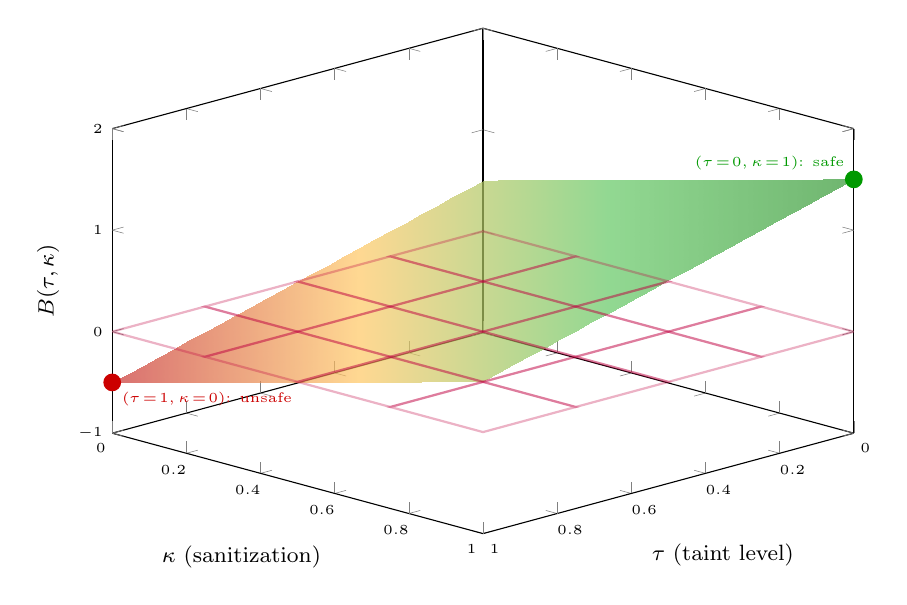
\begin{tikzpicture}
\begin{axis}[
  xlabel={$\tau$ (taint level)},
  ylabel={$\kappa$ (sanitization)},
  zlabel={$B(\tau, \kappa)$},
  view={135}{25},
  width=11cm, height=8cm,
  domain=0:1, y domain=0:1,
  zmin=-1, zmax=2,
  colormap={barrier}{
    rgb255(0cm)=(200,50,50);
    rgb255(0.333cm)=(255,200,100);
    rgb255(0.667cm)=(100,200,100);
    rgb255(1cm)=(50,150,50)
  },
  samples=25,
  xlabel style={font=\footnotesize},
  ylabel style={font=\footnotesize},
  zlabel style={font=\footnotesize},
  tick label style={font=\tiny},
]

% Barrier surface at block 4
\addplot3[surf, opacity=0.7, shader=interp]
  {(1-x) + y - 0.5};

% B = 0 plane
\addplot3[mesh, draw=purple, thick, domain=0:1, y domain=0:1,
  samples=5, opacity=0.3]
  {0};

% Initial state projection (tau=1, kappa=0)
\addplot3[only marks, mark=*, mark size=3pt, red!80!black]
  coordinates {(1, 0, -0.5)};
\node at (axis cs:1,0,-0.5) [anchor=north west, font=\tiny, red!80!black]
  {$(\tau\!=\!1, \kappa\!=\!0)$: unsafe};

% Reachable state at sink (tau=0, kappa=1)
\addplot3[only marks, mark=*, mark size=3pt, green!60!black]
  coordinates {(0, 1, 1.5)};
\node at (axis cs:0,1,1.5) [anchor=south east, font=\tiny, green!60!black]
  {$(\tau\!=\!0, \kappa\!=\!1)$: safe};

\end{axis}
\end{tikzpicture}
\caption{The barrier surface $B(\tau, \kappa) = (1-\tau) + \kappa -
  \tfrac{1}{2}$ at program counter $\pi=4$ (SQL sink).  The purple
  plane is $B=0$.  The reachable state (green, $\tau=0, \kappa=1$) lies
  above the barrier; the unsafe state (red, $\tau=1, \kappa=0$) lies
  below.  No execution path crosses from above to below.}
\label{fig:barrier-surface}
\end{figure}

%==============================================================================
\section{Step 4: SOS Certificate}
\label{sec:sos}
%==============================================================================

\subsection{From Barrier to Sum-of-Squares}

The barrier conditions require proving polynomial non-negativity over
semialgebraic sets.  By the Putinar Positivstellensatz
(as implemented in the A3 framework's \texttt{foundations.py} and
\texttt{positivstellensatz.py} modules), this reduces to a
\emph{sum-of-squares} (SOS) decomposition.

\begin{theorem}[SOS Encoding of Inductiveness]
\label{thm:sos}
The inductiveness condition for transition $T_{\text{sanitize}}$:
\[
  B(s) \geq 0 \;\wedge\; (s,s') \in T_{\text{san}}
  \implies B(s') \geq 0
\]
is equivalent to the non-negativity of:
\begin{equation}
  B(s') - \underbrace{\sigma_0(s,s')}_{\text{SOS}} \cdot B(s)
    - \underbrace{\sigma_1(s,s')}_{\text{SOS}} \cdot p_{T_{\text{san}}}(s,s')
    \;\geq\; 0
\end{equation}
where $\sigma_0, \sigma_1$ are SOS multiplier polynomials and
$p_{T_{\text{san}}}$ encodes the transition guard.
\end{theorem}

\subsection{Concrete SOS Decomposition}

For the sanitizer transition, the inductiveness check reduces to
verifying:
\begin{equation}
  (1 - \tau') + \kappa' - \tfrac{1}{2} \;\geq\; 0
  \quad\text{subject to}\quad
  \tau' = 0,\; \kappa' = 1
\end{equation}

Substituting:
\begin{equation}
  (1 - 0) + 1 - \tfrac{1}{2} = \tfrac{3}{2} \geq 0
\end{equation}

The SOS certificate is trivial (a positive constant):
\begin{equation}
  \sigma_0 = \tfrac{3}{2}, \quad \sigma_1 = 0
  \quad\Longrightarrow\quad
  \tfrac{3}{2} = \tfrac{3}{2} \cdot 1^2 \in \Sigma^2[\tau, \kappa]
\end{equation}

For the unsafe region check, we need
$-B(u) > 0$ when $\pi=4, \tau=1, \rho=0$:
\begin{equation}
  -B(u) = \tfrac{1}{2} - \kappa
  \quad\text{subject to}\quad
  \kappa \in \{0,1\},\; \kappa = 0
  \quad\Longrightarrow\quad
  \tfrac{1}{2} > 0. \quad\checkmark
\end{equation}

The SOS witness for $\tfrac{1}{2} - \kappa \geq 0$ on $\{\kappa = 0\}$:
\begin{equation}
  \tfrac{1}{2} - \kappa
    = \tfrac{1}{2} \cdot 1^2 + 1 \cdot (0 - \kappa)
    = \tfrac{1}{2} + \underbrace{\sigma_{\text{eq}}}_{\text{SOS=1}} \cdot
      \underbrace{h_{\text{eq}}}_{=-\kappa}
\end{equation}
confirming non-negativity via Putinar's representation.

%==============================================================================
\section{The Unsafe Variant: Certificate Refutation}
\label{sec:unsafe}
%==============================================================================

For comparison, consider the unsafe variant
(Listing~\ref{lst:unsafe}) where no sanitizer is called.  The
transition system changes: there is no $T_{\text{sanitize}}$, and
the format transition directly uses \texttt{raw\_name}:

\begin{align}
  T_{\text{format}}^{\text{unsafe}} &: (\pi=2) \;\longrightarrow\;
    (\pi'=3,\; \tau'=\tau,\; \kappa'=0,\; \rho'=0)
\end{align}

\begin{proposition}[No Barrier Exists for Unsafe Variant]
There is no polynomial $B$ satisfying the three barrier conditions for
the unsafe variant.
\end{proposition}

\begin{proof}
At $\pi=4$ (sink), the reachable state has $\tau=1, \kappa=0, \rho=0$,
which is exactly the unsafe region.  The reachable set intersects
$\Unsafe$:
\[
  \Reach \;\cap\; \Unsafe \;\neq\; \emptyset
\]
By the contrapositive of the barrier separation theorem
(Theorem~3.1 in the companion paper
\texttt{barrier-certificate-theory.tex}), no barrier certificate can
exist.  The verifier correctly reports: \textbf{SQL\_INJECTION}
at the \texttt{cursor.execute} call.
\end{proof}

%==============================================================================
\section{Why Barriers Succeed Where Others Fail}
\label{sec:comparison}
%==============================================================================

\subsection{Comparison Table}

\begin{table}[ht]
\centering
\renewcommand{\arraystretch}{1.3}
\begin{tabular}{@{}lcccc@{}}
\toprule
\textbf{Approach} &
\textbf{Proves safe?} &
\textbf{Compositional?} &
\textbf{Proof artifact?} &
\textbf{Scales interproc.?} \\
\midrule
Type checking &
\ding{55} &
\ding{51} &
Types &
\ding{51} \\
Abstract interp. &
\ding{55}\textsuperscript{a} &
\ding{55} &
Fixpoint &
\ding{55} \\
BMC ($k$-bounded) &
\ding{55}\textsuperscript{b} &
\ding{55} &
None &
\ding{55} \\
\textbf{Barrier certificate} &
\ding{51} &
\ding{51} &
Polynomial &
\ding{51} \\
\bottomrule
\end{tabular}

\medskip
\footnotesize
\textsuperscript{a} Fails because opaque sanitizer forces havoc
($\tau' = \top$). \\
\textsuperscript{b} Proves safety for $k$ steps only, not universally.

\caption{Comparison of verification approaches for SQL injection
  with sanitization.}
\label{tab:comparison}
\end{table}

\subsection{The Fundamental Limitation of Non-Barrier Approaches}

\begin{whybarrier}
\textbf{The conservatism trap.}  In the A3 framework's
\texttt{interprocedural\_taint.py} (around line~350), when a function's
parameter-to-sink mapping is unknown, the analysis conservatively
assumes \emph{all} parameters flow to all sinks:

\begin{lstlisting}[style=python, numbers=none, frame=none,
  backgroundcolor=\color{red!5}]
if not params_for_sink:
    params_for_sink = set(range(len(args)))  # ALL params might flow
\end{lstlisting}

This is sound but imprecise---it generates false positives whenever a
sanitizer intervenes.  The barrier certificate avoids this by proving
\emph{which} parameters don't flow, via a mathematical witness that
composes across call boundaries.

\medskip\noindent
\textbf{The expressiveness gap.}  The taint lattice
$\ell = (\tau, \kappa, \sigma)$ from \texttt{taint\_lattice.py} tracks:
\begin{itemize}[nosep]
  \item $\tau$: 16-bit source bitmask (which untrusted sources),
  \item $\kappa$: 32-bit sanitized-sinks bitmask (which sinks are safe),
  \item $\sigma$: 16-bit sensitivity bitmask (which secrets).
\end{itemize}
A type system can encode $\tau$ and $\sigma$ as phantom types, but
\emph{cannot} express $\kappa$ (``this value has been sanitized for
SQL but not for XSS'') because sanitization is a \emph{semantic}
property of program execution, not a syntactic property of types.  The
barrier certificate encodes this via the $\kappa$ coordinate in the
polynomial state space.
\end{whybarrier}

\subsection{Compositional Barrier Diagram}

\begin{figure}[ht]
\centering
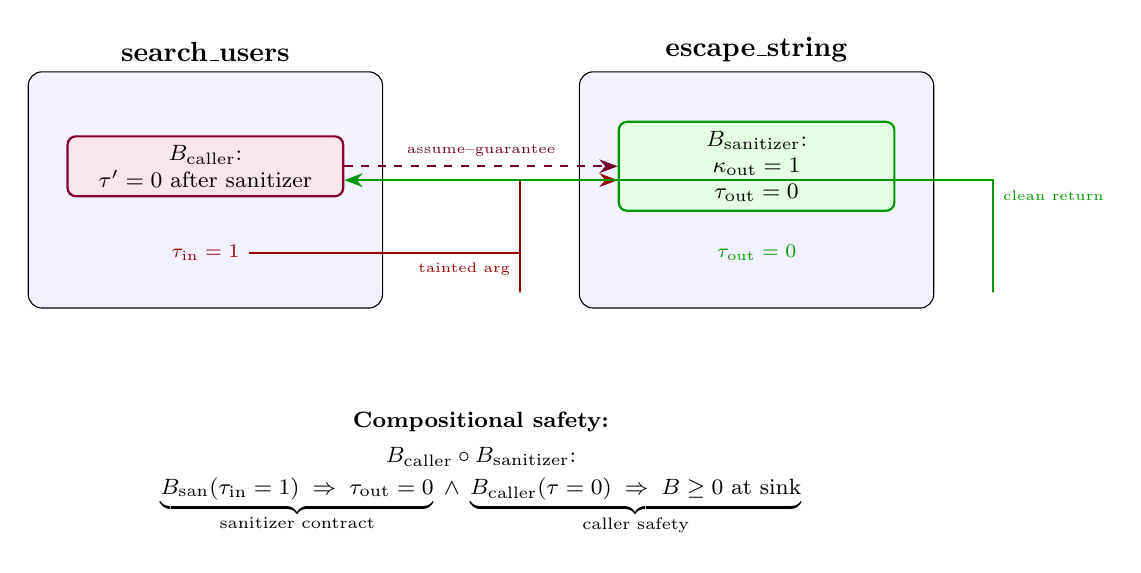
\begin{tikzpicture}[
  module/.style={
    rectangle, draw, rounded corners=5pt,
    minimum width=4.5cm, minimum height=3cm,
    font=\small, fill=blue!5
  },
  barrier/.style={
    rectangle, draw=purple!70!black, thick,
    rounded corners=3pt, fill=purple!10,
    font=\footnotesize, align=center,
    minimum width=3.5cm
  },
  arr/.style={-Stealth, thick},
  contract/.style={-Stealth, thick, dashed, purple!60!black}
]

% Module boxes
\node[module] (M1) at (0,0) {};
\node[above] at (M1.north) {\textbf{search\_users}};

\node[module] (M2) at (7,0) {};
\node[above] at (M2.north) {\textbf{escape\_string}};

% Barrier boxes inside modules
\node[barrier] (B1) at (0, 0.3) {
  $B_{\text{caller}}$:\\
  $\tau' = 0$ after sanitizer
};
\node[barrier, draw=green!60!black, fill=green!10] (B2) at (7, 0.3) {
  $B_{\text{sanitizer}}$:\\
  $\kappa_{\text{out}} = 1$\\
  $\tau_{\text{out}} = 0$
};

% Flow arrows
\node[font=\scriptsize, red!60!black] (tin) at (0, -0.8)
  {$\tau_{\text{in}} = 1$};
\node[font=\scriptsize, green!60!black] (tout) at (7, -0.8)
  {$\tau_{\text{out}} = 0$};

% Contract arrows
\draw[contract] (B1.east) -- node[above, font=\tiny]
  {assume--guarantee} (B2.west);
\draw[arr, red!60!black] (tin) -| node[below left, font=\tiny]
  {tainted arg} (4, -1.3) |- ([yshift=-5pt]B2.west);
\draw[arr, green!60!black] ([yshift=-5pt]B2.east) -|
  (10, -1.3) |- node[below right, font=\tiny] {clean return}
  ([yshift=-5pt]B1.east);

% Composition equation
\node[below=1.5cm of M1, font=\footnotesize, align=center] (eq) at (3.5, -1.2) {
  \textbf{Compositional safety:} \\[3pt]
  $B_{\text{caller}} \circ B_{\text{sanitizer}}$: \\[2pt]
  $\underbrace{B_{\text{san}}(\tau_{\text{in}}=1)
    \;\Rightarrow\; \tau_{\text{out}}=0}_{\text{sanitizer contract}}
  \;\wedge\;
  \underbrace{B_{\text{caller}}(\tau=0)
    \;\Rightarrow\; B \geq 0 \text{ at sink}}_{\text{caller safety}}$
};

\end{tikzpicture}
\caption{Compositional barrier certificates across function boundaries.
  The sanitizer module provides a contract
  ($\tau_{\text{out}}=0$), and the caller's barrier relies on this
  contract.  No inlining is needed.}
\label{fig:compositional}
\end{figure}

%==============================================================================
\section{Complete Formal Summary}
\label{sec:summary}
%==============================================================================

\begin{pipelinebox}
\begin{enumerate}[leftmargin=*]
\item \textbf{Python source} (Listing~\ref{lst:target}):
  \texttt{search\_users(request, cursor)} with HTTP input, sanitizer, SQL sink.

\item \textbf{Bytecode extraction}: CPython 3.12+ dis module $\to$
  27 instructions across 6 basic blocks.

\item \textbf{CFG construction} (Figure~\ref{fig:cfg}): 6 blocks,
  taint source at $B_0$, sanitizer at $B_2$, sink at $B_4$.

\item \textbf{Taint-augmented state space}:
  $s = (\pi, \tau, \kappa, \nu, \rho) \in \R^5$.

\item \textbf{Semialgebraic encoding}:
  \begin{align*}
    \Init &= \{\pi=0, \tau=1, \kappa=0, \nu\in\{0,1\}, \rho=0\} \\
    \Trans &= T_{\text{src}} \vee T_{\text{guard}} \vee
      T_{\text{san}} \vee T_{\text{fmt}} \vee T_{\text{exec}} \\
    \Unsafe &= \{\pi=4, \tau=1, \rho=0\}
  \end{align*}

\item \textbf{Barrier certificate}:
  \[
    B(s) = \sum_{k=0}^{5} \ell_k(\pi) \cdot B_k(\tau, \kappa)
    \quad\text{with}\quad
    B_4 = (1-\tau) + \kappa - \tfrac{1}{2}
  \]

\item \textbf{Verification}:
  \begin{itemize}[nosep]
    \item Initial: $B(s_0) = 1 \geq 0$ \checkmark
    \item Inductive: verified for all 6 transitions \checkmark
    \item Unsafe: $B(u) = -\tfrac{1}{2} < 0$ \checkmark
  \end{itemize}

\item \textbf{SOS witness}: $B_4 = \tfrac{3}{2} \cdot 1^2 \in
  \Sigma^2[\tau,\kappa]$ at reachable sink states.

\item \textbf{Conclusion}: \texttt{search\_users} is \textbf{safe}
  from SQL injection (CWE-089).
\end{enumerate}
\end{pipelinebox}

\subsection{Contrast: Why This Cannot Be Done Without Barriers}

The barrier certificate provides three properties that no other single
technique achieves simultaneously:

\begin{enumerate}
\item \textbf{Semantic taint tracking embedded in $\R^n$}:
  The $\tau$ coordinate distinguishes tainted from clean values
  within the \emph{same} Python type.  Type systems cannot refine
  \texttt{str} this way.

\item \textbf{Inductive compositional proof}:
  The barrier composes across \texttt{escape\_string} via an
  assume-guarantee contract on $\kappa$ and $\tau$.  Abstract
  interpretation cannot compose across opaque functions without
  inlining or conservative havoc.

\item \textbf{SOS-checkable artifact}:
  The polynomial certificate $B$ and its SOS decomposition can be
  independently verified by any SDP solver (or even by hand for
  small degrees).  BMC traces are not reusable proof objects.
\end{enumerate}

These properties make barrier certificates the \emph{only} approach
that can prove interprocedural taint safety with opaque sanitizers
while producing a machine-checkable mathematical proof.

%==============================================================================
\section{Connection to the A3 Codebase}
\label{sec:codebase}
%==============================================================================

\begin{table}[ht]
\centering
\renewcommand{\arraystretch}{1.2}
\begin{tabular}{@{}ll@{}}
\toprule
\textbf{Pipeline stage} & \textbf{A3 module} \\
\midrule
Bytecode analysis & \texttt{a3\_python/semantics/crash\_summaries.py} \\
CFG construction & \texttt{a3\_python/cfg/control\_flow.py} \\
State encoding ($s \to$ Z3) & \texttt{a3\_python/barriers/step\_relation.py} \\
Guard $\to$ barrier translation & \texttt{a3\_python/barriers/guard\_to\_barrier.py} \\
Taint lattice $(\tau,\kappa,\sigma)$ & \texttt{a3\_python/z3model/taint\_lattice.py} \\
Source/sink contracts & \texttt{a3\_python/contracts/security\_lattice.py} \\
Intraprocedural taint & \texttt{a3\_python/semantics/intraprocedural\_taint.py} \\
Interprocedural taint & \texttt{a3\_python/semantics/interprocedural\_taint.py} \\
Barrier synthesis & \texttt{a3\_python/semantics/interprocedural\_barriers.py} \\
SOS / Positivstellensatz & \texttt{a3\_python/barriers/foundations.py} \\
Polynomial certificates & \texttt{a3\_python/barriers/sos\_safety.py} \\
SQL injection predicates & \texttt{a3\_python/unsafe/security/sql\_injection.py} \\
\bottomrule
\end{tabular}
\caption{Mapping from pipeline stages to A3 codebase modules.}
\label{tab:codebase-map}
\end{table}

\end{document}
